\documentclass[../full_thesis/full_thesis.tex]{subfiles}

% Default image directory
\newcommand{\thisdir}{../detecting_cgw}
\graphicspath{{\thisdir/img/}}

\begin{document}

Timing variations, in the form of glitches or timing noise, may pose a serious
risk to efforts to discover continuous GWs from neutron stars. This is because
searches rely on \emph{matched filtering}, which searches the data using a
template; if the template and signal don't match, due to timing variations in
the signal, the template may be unable to detect the signal. In this section,
we will give a general introduction to the detection methods used in GW data
analysis and then develop our tools which will used in later chapters to
quantify the significance of timing variations for continuous GW searches. The
details of estimating the risk posed by glitches to GW searches will be
discussed in Chapter~\ref{sec: glitches in cgw} and then in Chapter~\ref{sec:
timing noise in cgw} and Chapter.~\ref{sec: timing noise in cgw analytic} we
will investigate the role of timing noise for GW searches.

\section{Introduction}
\label{sec: introduction cgw}
Rotating neutron stars capable of supporting non-axisymmetric mass
distributions will emit continuous gravitational
waves\footnote{Note that in general `continuous waves' can
    refer to any quasi-monochromatic long-lasting gravitational-wave
        signals, such as emitted by binaries of white dwarfs, neutron
        stars or black holes, which would be detectable by LISA or pulsar
        timing arrays. Here we refer to continuous GWs exclusively in the context of
        spinning nonaxisymmetric neutron stars as relevant to ground-based
        detectors.}
(GWs) due to their
time-varying quadrupole moments. These may be detectable by ground-based detectors. The emitted
signals can persist for longer than
typical search durations, but are weak in amplitude, making them difficult to detect
in the noise of the detector.

To find a signal, continuous GW searches use matched
filtering techniques such as the $\mathcal{F}$-statistic \citep{Jaranowski1998},
which compare the output of the detector with a template.  These techniques are
powerful, provided that the signal and template remain coherent for the duration
of the observation. If the signal can be perfectly matched by a template then
the signal to noise ratio, used to quantify the detection likelihood, scales as
$\rho^{2} \propto \To$ (e.g.\ see~\citep{Prix2009}). This suggests searching
over longer observations increases the chances of making a detection.

The templates must model the monotonic spin-down of the source due to the
electromagnetic (EM) and gravitational torque; this is done by Taylor expanding
the phase (see Eqn.~\eqref{eqn: Taylor compact}) about some reference time
$\tref$.
%\begin{equation}
%\Phi(t) = \phi_{0} + 2\pi\left(\f_{0} (t - \tref) +
%          \frac{\fdot_{0}}{2!} (t - \tref)^{2}
%           %+ \frac{\fddot}{3!} (t - t_{i})^{3}
%           \right)
%           + \ldots
%           \,,
%\label{eqn: Taylor}
%\end{equation}
%$\tref$ is the reference time at which the pulsar frequency and
%spin-down parameters $[\phi_{0}, \f_{0}, \fdot_{0}, \ldots]$ are defined.

Note that all times refer to the solar system barycentre and we assume the
timing model has already correctly accounted for the dispersion measure, proper
motion and other parameters as discussed in \citet{Edwards2006}.  Pulsar
astronomers fit this model to observed time of arrivals (TOAs). If the best fit
model is accurate enough to track the pulsar to within a single rotation, the
resulting timing solution is described as \emph{phase-connected}.  Often such
solutions are capable of tracking the pulsar over durations greater than  a
year \citep{Lyne2012book}.  For gravitational-wave searches, this level of
accuracy motivates the use of the same Taylor expansion phase models to account
for the spin-down.  Pulsar astronomers measure the frequency $\nu$ and higher
order coefficients describing the rotation of the pulsar itself. In this work
we will denote the GW frequency and its derivatives by $f, \dot{f}$, etc.\ The relation between the GW frequency and rotation frequency depends on
the emission mechanism; in this work we will consider only searches for emission from
non-axisymmetric neutron stars such that $f=2\nu$~\citep{Shapiro83}.

The rest of this chapter is organised as follows: in Section~\ref{sec:
introduction to the mismatch} we will define the mismatch which
quantifies the loss of signal to noise ratio for imperfectly matched signals.
In Section~\ref{sec: mismatch from differences in the gw phase} we will
familiarise the reader with methods to calculate the mismatch when the phase of
the GW is not a smooth Taylor expansion and describe why this method of
calculating the mismatch becomes intractable for complicated signals. Then, in
Section~\ref{sec: generalising the metric-mismatch} we will define a new approach
to calculating the mismatch by splitting the signal into separate subdomains.


\section{Introduction to the mismatch}
\label{sec: introduction to the mismatch}
While Taylor expansion models are on average reliable enough to track the
spin-down, pulsars do show timing variations either in the form of glitches,
occasional sudden increases in the rotation frequency, or continuous
low-frequency variations known as \emph{timing noise} (see Chapter~\ref{sec:
timing variations} for an overview). To quantify the effect these variations
will cause, we will use the \emph{mismatch}, which is the loss of signal to
noise ratio due to the imperfect matching the template and the signal. The
mismatch is non-zero whenever the signal and template are not perfectly
matched. Even if the signal does not contain any timing variations a mismatch
can occur when the template, chosen from a finite grid of points in parameter
space, does not share exactly the same parameters as the signal. This problem
has been studied in detail since finite computing resources limit the number of
templates that can be used in a search ensuring that any prospective search
must have some level of mismatch. In this section, we introduce the tools
that have been developed to understand this problem. We will return to the
problem of timing variations later on in this chapter.

\subsection{Defining the mismatch}

We begin by assuming that the gravitational-wave detector strain data contains
a periodic GW signal with phase $\PhiS(t; \ls^{\alpha})$, where $\ls^{\alpha}$
is a vector of the signal parameters. A fully-coherent search consists of
applying a matched filtering algorithm over a coherence time $\Tcoh$ to search
the data using a \emph{template}; let us then denote the phase evolution of the
template as $\PhiT(t; \lt^{\alpha})$, such that $\lt^{\alpha}$ is a vector of
the template parameters.

Defining the phase-difference between the signal and the template as
\begin{align}
\Delta\Phi(t; \lt^{\alpha}, \ls^{\alpha}) = \PhiS(t; \ls^{\alpha}) - \PhiT(t; \lt^{\alpha}),
\label{eqn: phase diff}
\end{align}
then, following the work of \citet{Prix2005} and neglecting amplitude modulations
in the signal, we can define the matched filtering amplitude
\begin{equation}
X %= \frac{1}{\Tcoh}\int e^{i\PhiS(t)} e^{-i\PhiT} dt
= \frac{1}{\Tcoh}\int_{\Tcoh}e^{i\Delta\Phi} dt,
\label{eqn: matched filtering amplitude}
\end{equation}
This amplitude will have a global maximum of $|X|=1$ for a perfectly matched
signal and will decrease for increasing phase mismatches. In this way, if we
define $\rhotilde$ as the signal to noise ratio (SNR) measured in a fully-coherent
search, then $X$ defines the loss of SNR incurred
due to the non-zero phase difference $\Delta\Phi$ as compared to a perfectly matched signal
with SNR $\rhotilde_{\textrm{pm}}$ such that
\begin{align}
\rhotilde = |X|\rhotilde_{\textrm{pm}}%.
\end{align}
A simple, dimensionless measure of the loss of SNR is found by rearranging
and defining the fully-coherent \emph{mismatch} as
\begin{equation}
\mutilde(\ls^{\alpha}, \lt^{\alpha}) = 1 - |X(\ls^{\alpha}, \lt^{\alpha})|^{2},
\label{eqn: full mismatch}
\end{equation}
such that
\begin{equation}
\mutilde = \frac{\rhotilde_{\mathrm{pm}}^{2} - \rhotilde^{2}}
                {\rhotilde^{2}_{\mathrm{pm}}}.
\label{eqn: numeric mismatch}
\end{equation}

\subsection{Interpreting the mismatch}
In this work we will quantify the effect of glitches by the mismatch. However,
it may be useful to interpret a mismatch in the following way. For a perfectly
matched continuous GW signal it can be shown \citep{Jaranowski1998} that the SNR scales as
\begin{equation}
\rho_{\mathrm{pm}} \propto \frac{h_{0}}{\sqrt{\textrm{S}_{\textrm{n}}}}
                               \sqrt{\Tobs \mathcal{N}},
\end{equation}
where $h_{0}$ is the strain-amplitude for an optimally oriented source with
respect to the detector, $\sqrt{\textrm{S}_{\textrm{n}}}$ the noise measured
in the detector and $\mathcal{N}$ is the number of detectors.

Combining this equation with Eqn.~\eqref{eqn: numeric mismatch}, the SNR of a signal
with fully-coherent mismatch $\mutilde$ scales as
\begin{equation}
\rho \propto \sqrt{1-\mutilde} \frac{h_{0}}{\sqrt{\textrm{S}_{\textrm{n}}}}
                               \sqrt{\Tobs \mathcal{N}},
\end{equation}
which is to say it reduces the sensitivity by a factor~$\sqrt{1-\mutilde}$.



\subsection{Taylor expansion signals and templates}
So far we have not yet defined a phase evolution model for either the signal or the template.
The signal phase $\PhiS(t; \ls^{\alpha})$ will depend on the GW production mechanism,
but assuming the signal is generated by the canonical non-axisymmetric distortion,
the GW signal will be produced at twice the rotation frequency and spin-down
with twice the rotational spin-down rate. From the success of pulsar astronomy,
we know that the phase evolution of the rotation can be modelled by a Taylor
expansion, typically up to the first order in frequency derivative. Therefore,
we can begin by modelling the GW phase evolution using a Taylor expansion
\begin{equation}
\PhiS (t, \ls^{\alpha}) = \phiS + 2\pi \left(\nuS (t - \tref)
+ \frac{\nudotS}{2}(t - \tref)^{2} \right),
\label{eqn: Taylor lambda signal}
\end{equation}
such that $\ls^{\alpha} = [\phiS, \nuS, \nudotS]$. In principle, we can include
higher order terms, but for this work we truncate at the first
derivative of the frequency.

For blind searches, where we have no hints about the phase evolution,
typical continuous GW searches assume that the GW signal is a Taylor expansion and
search for it using a Taylor expansion template. Defining $\lt^{\alpha} = [\phiT,
\nuT, \nudotT]$ as the Taylor expansion
template parameters, Eqn.~\eqref{eqn: phase diff}, the phase difference, is
\begin{align}
\Delta \Phi(t; \ls^{\alpha}, \lt^{\alpha})  & =
\Deltaphi + 2\pi\left(\Deltanu(t-\tref) +
\frac{\Deltanudot}{2}(t - \tref)^{2}\right),
\label{eqn: Delta Phi}
\end{align}
where $\dl^{\alpha} = \ls^{\alpha} - \lt^{\alpha}$. Note that
by choosing any two of $\ls^{\alpha}, \lt^{\alpha}$, and $\dl^{\alpha}$
we have a choice of three equivalent parameterisations.
When the parameter offset $\dl^{\alpha}$ vanishes, the matched filtering
amplitude tends to unity and hence the mismatch tends to zero. In the other
extreme, for a suitably
large parameter space offsets the mismatch approaches zero and so the signal is
completely lost.

Substituting Eqn.~\eqref{eqn: Delta Phi} into Eqn.~\eqref{eqn: full mismatch}
gives the mismatch between a smooth Taylor expansion signal and template. In
this work we will calculate the mismatch for a signal that is not a smooth
Taylor expansion. This can be done in this way for some special cases. For
example, taking $\dl^{\alpha} = [\Deltaphi, 0, 0]$, the mismatch is found to be
zero: this reflects the fact that fully-coherent matched filtering is
insensitive to any arbitrary phase offset between the signal and template. In
more complicated cases, the integrals become intractable. To aid in
calculation, we will use the so-called metric approximation. In the next section
we will introduce it in the context of smooth Taylor expansion signals, later on
in Section~\ref{sec: generalising the metric-mismatch} we will describe how we
extend it to arbitrary signals.

\subsection{The metric-mismatch approximation for fully-coherent searches}
\label{sec: the metric-mismatch approximation for fully-coherent searches}

The fully-coherent mismatch Eqn.~\eqref{eqn: full mismatch} has a local
minimum of zero at $\dl^{\alpha}=0$. Expanding about this minimum up to the
leading order term, \citet{Brady1998} approximated the mismatch by
\begin{equation}
\mutilde(\lt^{\alpha}, \dl^{\alpha}) \approx
g_{\alpha\beta}\dl^{\alpha}\dl^{\beta},
\label{eqn: mismatch metric single}
\end{equation}
where $g_{\alpha\beta}$ is the parameter space metric given by
\begin{equation}
    g_{\alpha\beta} =
    \frac{1}{2}\partial_{\alpha}\partial_{\beta}
    \mutilde(\lt^{\alpha}, \dl^{\alpha}) \biggr\rvert_{\dl^{\alpha}=0}.
\end{equation}
Note that we define $\partial_{\alpha} \equiv \partial_{\dl^{\alpha}}$.
The metric is a function  of both the total coherence time~$\Tcoh$ over which the
matched filter is performed and the reference time at which the Taylor expansions
are defined, but not the signal itself. Partially evaluating the metric, we find that
\begin{align}
\begin{split}
    g_{\alpha \beta} = &
    \frac{1}{\Tcoh}\int_{0}^{\Tcoh}\partial_{\alpha}\Delta\Phi
                               \partial_{\beta}\Delta\Phi dt \\
   & -\frac{1}{\Tcoh^{2}}\int_{0}^{\Tcoh} \partial_{\alpha}\Delta\Phi dt
                 \int_{0}^{\Tcoh} \partial_{\beta}\Delta\Phi dt.
\end{split}
\label{eqn: fully-coherent metric simple}
\end{align}

This metric formulation provides a method to measure the \emph{metric-mismatch} between a
signal and template that are both Taylor expansions. \citet{Brady1998} proposed
this method with the aim of picking the spacing of templates in parameter space
such that the maximum allowable mismatch would not rise above a pre-defined
threshold. In this work, we will instead use this metric-mismatch approximation to
calculate mismatches between signals and Taylor expansion templates.

It is worth commenting that the full mismatch, as calculated from
Eqn.~\eqref{eqn: full mismatch}, is bounded by $[0, 1]$. In contrast, the
approximate metric-mismatch is bounded by $[0, \infty)$. This is because the
expansion of the mismatch in Eqn.~\eqref{eqn: mismatch metric single} was
taken about $\Delta\lambda^{\alpha}=0$ and so for sufficiently large parameter
space offsets the expansion breaks down. In this case, the metric-mismatch
approximation non-linearly overestimates the true mismatch. A metric-mismatch
above one, while losing the interpretation as a direct loss of SNR, still
corresponds to a large true mismatch, and hence a significant loss of SNR.

%\meta{Greg: Reinhard is there a reference to Karl's work on this?}

\subsection{The mismatch for semi-coherent searches}
\label{sec: semi-coherent mismatch}

Fully-coherent searches are computationally demanding, so much so that it is
infeasible to perform fully-coherent searches for wide-parameter searches
such as the all-sky search. Instead, \emph{semi-coherent}
searches are used which require far fewer templates and result in more
sensitive searches at a fixed computing cost \citep{Prix2009}. There are numerous
implementations of semi-coherent searches, for example the E@H search uses
the Hough-transform method \citep{Krishnan2004}; in this section we will discuss
the generic case.

A semi-coherent search divides an observation time $\Tobs$ into $\Nseg$ segments of
duration $\Tcoh$. Each segment is searched fully coherently with a resulting
SNR $\rhotilde^{2}_{j}$ where $j$ labels the
segment. The semi-coherent search then recombines these segments by summing
all segments at the same point in parameter space $\lt^{\alpha}$ to give a new
detection statistic
\begin{align}
\rhohat^{2}(\lt^{\alpha}, \dl^{\alpha}) =
 \sum_{j}^{\Nseg}\rhotilde^{2}_{j}(\lt^{\alpha}, \dl^{\alpha}),
\label{eqn: semi-coherent sum}
\end{align}
where the `hat' denotes that it is a semi-coherent quantity.

For each fully-coherent segment, we can rearrange Eqn.~\eqref{eqn: numeric mismatch}
to give
\begin{align}
\rhotilde^{2}_{j}(\lt^{\alpha}, \dl^{\alpha}) =
 \rhotilde^{2}_{\mathrm{pm}}(1 - \mutilde_{j}(\lt^{\alpha}, \dl^{\alpha})).
\end{align}
Here we take $\rhotilde_{\mathrm{pm}}$ to be the same for all segments such that
it does not carry a $j$-index; in this way we neglect variations
in the signal such as the signal amplitude or the motion of the Earth and also require
all segments to be of equal duration.
For the semi-coherent
detection statistic we may define $\rhohat^{2}_\mathrm{pm}$ as the squared SNR in the
absence of any mismatch. Then the semi-coherent mismatch $\muhat$ can be implicitly
defined as
\begin{align}
\rhohat^{2}(\lt^{\alpha}, \dl^{\alpha}) =
 \rhohat^{2}_\mathrm{pm}(1 - \muhat(\lt^{\alpha}, \dl^{\alpha})),
\end{align}
where $\muhat$ is the semi-coherent mismatch.
When there is no mismatch, the sum of the $\rhotilde^{2}_{\mathrm{pm}}$ is equal the
semi-coherent $\rhohat^{2}_{\mathrm{pm}}$ such that
\begin{align}
\rhohat^{2}_\textrm{pm} = \Nseg\rhotilde^{2}_\textrm{pm}.
\end{align}
Inserting all these expressions into Eqn.~\eqref{eqn: semi-coherent sum} we see that
the semi-coherent mismatch is an average over the individual full-coherent segment
mismatches:
\begin{align}
\muhat(\lt^{\alpha}, \dl^{\alpha}) =
 \frac{1}{\Nseg}\sum_{j=1}^{\Nseg}\mutilde_{j}(\lt^{\alpha}, \dl^{\alpha}).
\label{eqn: semi-coherent mismatch}
\end{align}

With this expression, we can first calculate the mismatch for each fully-coherent
segment, and then calculate the mismatch for a semi-coherent search. However, we
must be careful to sum all the mismatches at the same point in parameter space.

In this section we have introduced: the fully-coherent mismatch, used to
quantify the loss of SNR in fully-coherent GW searches; the metric-mismatch
approximation, a useful way to calculate mismatches that avoids the complicated
integration; and the semi-coherent mismatch, quantifying the loss of SNR in
semi-coherent GW searches. The mismatch is a useful way to quantify how well a
search performs given a particular GW signal. However, the tools discussed in
this section to calculate this mismatch apply only to smooth Taylor expansion
signals and templates. Signals which contain timing variations are by definition
not smooth Taylor expansions. Therefore, we need a method to calculate the
mismatch for arbitrary signals. In the next section, we will discuss some
special cases of timing variations where the mismatch can be calculated
exactly. Then in the final section, we will introduce a new tool which can be
used to calculate the mismatch for arbitrary signals.

\section{Exact mismatch from irregularities in the phase}
\label{sec: mismatch from differences in the gw phase}

The $\mathcal{F}$-statistic considered in \citet{Brady1998} analytically
minimises over the phase. Therefore, if the signal and template can both be
modelled by a single smooth Taylor expansion, but with a finite phase-offset,
the mismatch is zero: the mismatch is insensitive to any overall phase
difference between the signal and template. However, a mismatch will occur if
the overall phase between the signal and template changes during an
observation. In this section, we will investigate three scenarios where this
occurs. While not all these scenarios are physically relevant to real astrophysical
systems, this introduces some concepts in a simple setting before we tackle
the more difficult real astrophysical systems.

\subsection{Two subdomains with a phase discontinuity}
\label{sec: Two segments with a phase offset}

We begin with a simple system in which the signal undergoes an instantaneous
`jump' in its GW phase halfway through the observation. We can model this
signal by a \emph{piecewise} Taylor expansion with two subdomains.  Both
subdomains are of equal duration and follow a smooth spin-down, except that
there is a phase discontinuity at their interface; we illustrate this setup in
Figure~\ref{fig: PhaseJump}.
\begin{figure}[htb]
    \centering
    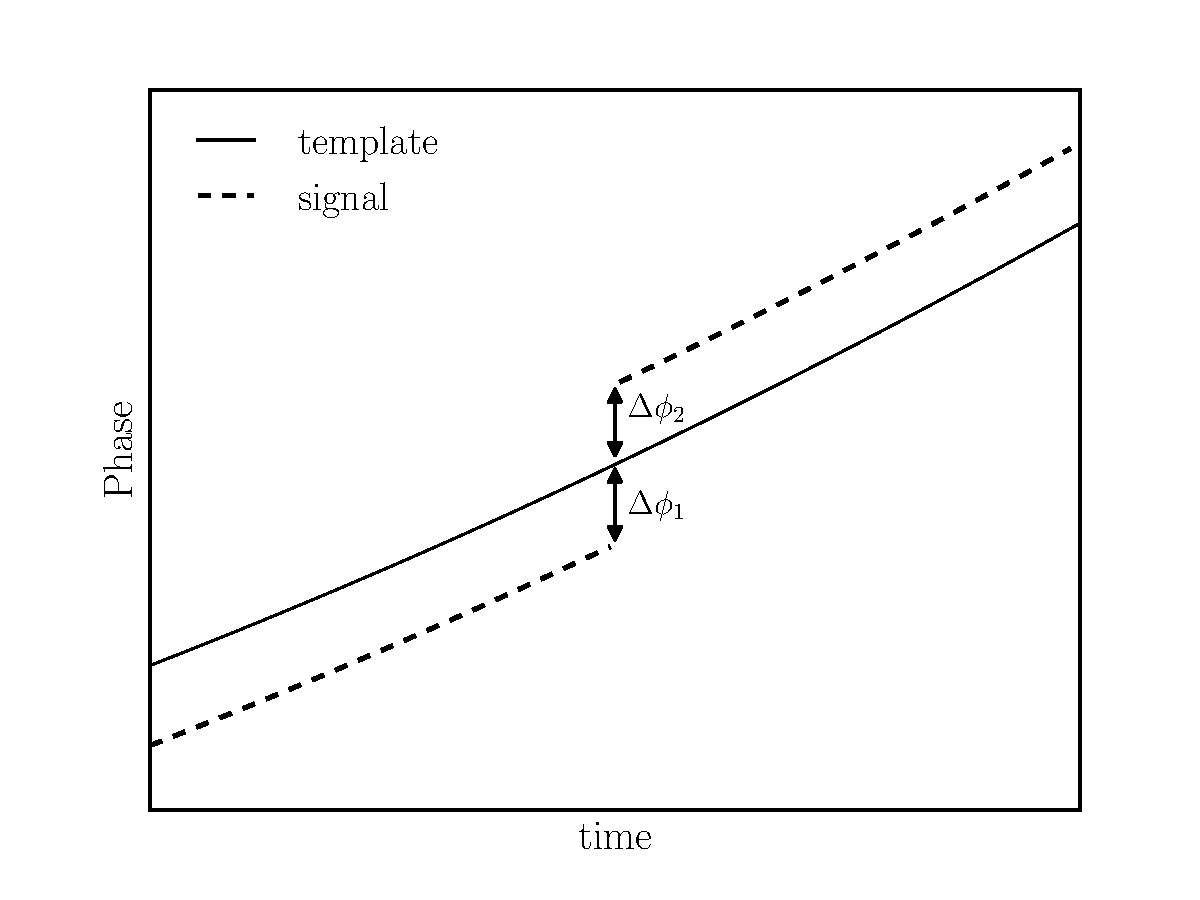
\includegraphics[width=.5\textwidth]{PhaseJump}
    \caption{Illustration of the signal and template defined in equation
        \eqref{eqn: phase offset}}
    \label{fig: PhaseJump}
\end{figure}
Parameterising by the offset with respect to the template parameters $\bl_{0}$ for some
arbitrary template and phase jump, we write the phase deviations in the two
subdomains as
\begin{equation}
 \Delta\Phi(t) = \left\{
\begin{array}{cr}
\Delta \phi_{1}& \; 0 < t < T/2 \\
\Delta \phi_{2} & \;  T/2 < t < T
\end{array}.
\right.
\label{eqn: phase offset}
\end{equation}

To compute the matched filtering amplitude given in Eqn.~\eqref{eqn: matched
filtering amplitude}, we can factorise the integral using the additivity of
integration on intervals into two integrations
\begin{eqnarray}
X & = &\frac{1}{T } \int_{0}^{T}e^{i\Delta\Phi(t)} dt\\
 & = &\frac{1}{T }\left(\int_{0}^{T /2}e^{i\Delta\phi_{1}} dt  +
\int_{T/2}^{T} e^{i\Delta\phi_{2}}dt\right)\\
& = & \frac{1}{2}\left(e^{i\Delta\phi_{1}} + e^{i\Delta\phi_{2}}\right).
\end{eqnarray}
Because our choice in splitting up the integral exactly matches the subdomains
defined in Eqn.~\eqref{eqn: phase offset} and in each subdomain $\Delta\Phi(t)$
is constant, we can compute the integrals.
The absolute square value of the matched filtering amplitude is then
\begin{eqnarray}
|X|^{2}& = &\frac{1}{4}\left(e^{i\Delta\phi_{1}} + e^{i\Delta\phi_{2}}\right) \left(e^{-i\Delta\phi_{1}} + e^{-i\Delta\phi_{2}}\right)\\
& = &\frac{1}{4} \left(2 + e^{i(\Delta\phi_{1} - \Delta \phi_{2})} +  e^{-i(\Delta\phi_{1} - \Delta_{\phi_{2}})} \right) \\
& = &\frac{1}{2}\left(1 + \cos(\Delta\phi_{1} - \Delta\phi_{2})\right).
\end{eqnarray}
Finally, the fully-coherent mismatch can be calculated from Eqn.~\eqref{eqn: full mismatch}
to be
\begin{equation}
\mutilde = \frac{1}{2}\left(1 - \cos(\Delta\phi_{1} - \Delta\phi_{2})\right).
\label{eqn: two segment phase mismatch}
\end{equation}

From this result, we learn that it is not the phase difference with respect to
each of the Taylor expansions ($\Delta\phi_1$ or $\Delta\phi_2$) that is
important, but the total phase jump at their interface. For $\Delta \phi_{1} =
\Delta \phi_{2}$ the mismatch vanishes, this recovering the case of a single
Taylor expansion signal with an arbitrary overall phase offset, which always has
zero mismatch. This result can be used to calculate the mismatch due to a glitch,
if the glitch is purely in the phase. In reality, we know that glitches are
discontinuities in the frequency and spin-down rate, this will be discussed later
in Chapter~\ref{sec: glitches in cgw}, but this simple calculation provides
a stepping stone to understanding the more complicated complete result.

%\paragraph{Comparing with an exact numerical result}
%\meta{Greg: potentially cut this} We can verify equation
%\eqref{eqn: two segment phase mismatch} by comparing with the results of a
%exact numerical calculation of the mismatch. This involves defining the signal
%such that it describes two segments with a phase offset, then `injecting' and
%recovering the signal using \texttt{LALApps} software. We do this in the
%absence of noise and compute the mismatch against a perfectly matched signal.
%The signal comprises two adjacent transient windows of fixed duration. We set
%the phase offset in the first segment to zero and subject the second segment to
%a phase jump $\Delta \phi$, therefore
%\begin{align}
%    \Delta \phi_{1} &= 0 &  \textrm{ and } && \Delta \phi_{2} =& \Delta\phi.
%\end{align}
%Varying $\Delta\phi$ we plot the exact numerical result along with the
%prediction of Eqn.~\eqref{eqn: two segment phase mismatch} in
%Figure~\ref{fig: two plot}
%\begin{figure}
%\centering
%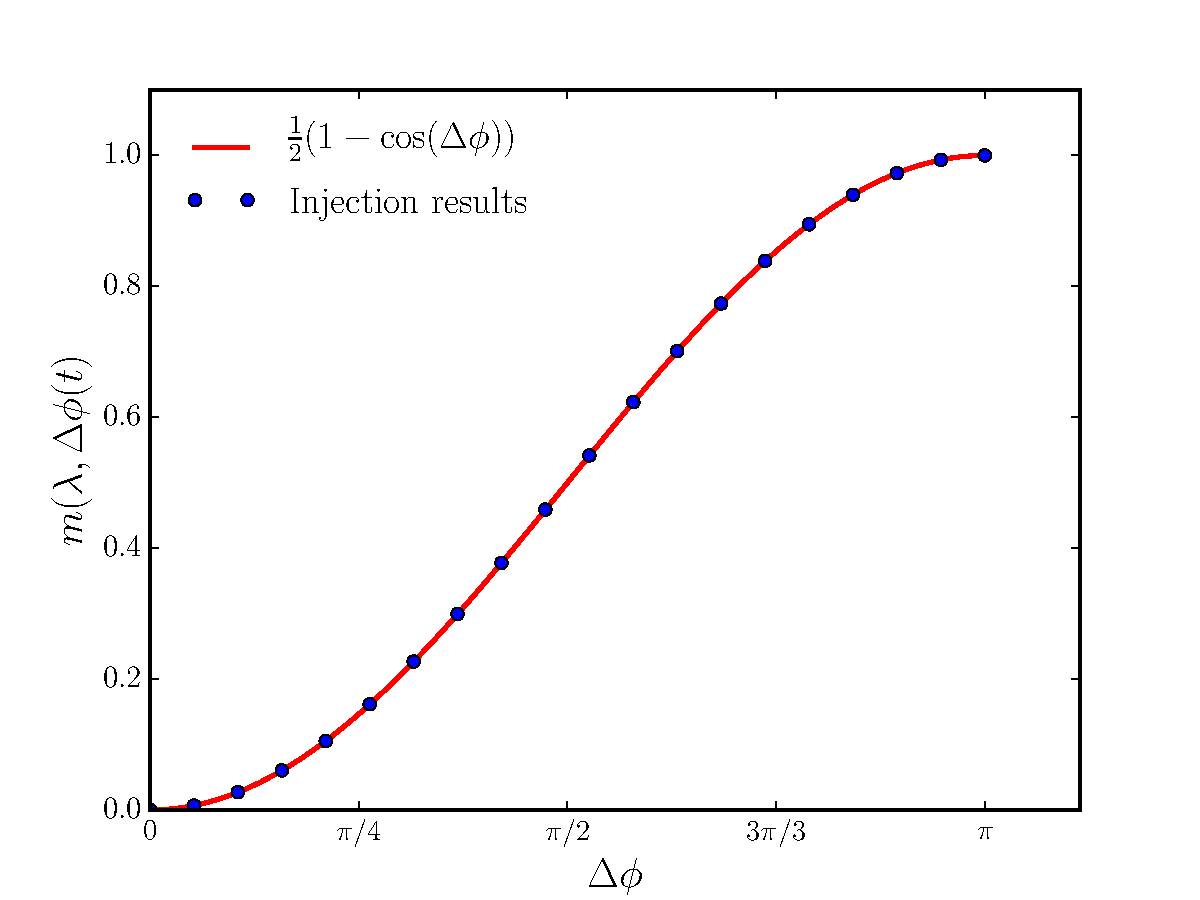
\includegraphics[width=0.65\textwidth]{Exact_analytic_phase_two_segments}
%\caption{Plot of the theoretical prediction of Eqn.~\eqref{eqn: two segment
%phase mismatch} given a time dependent phase offset as in equation\eqref{eqn:
%phase offset}. This is compared  with a signal injection and recovery
%using \texttt{LALapps} software.}
%\label{fig: two plot}
%\end{figure}

\subsection{N subdomains with phase discontinuities}
We can further generalise Eqn.~\eqref{eqn: two segment phase mismatch} by
letting the signal be comprised of $N$ equal duration subdomains with a phase discontinuity
$\Delta\phi_i$ for the $i^{th}$ subdomain.
Then, the matched filtering amplitude can be written
\begin{eqnarray}
X & = & \frac{1}{T}\left(\int_{0}^{t_{1}}e^{i\Delta\phi_{1}} dt +
\int_{t_{1}}^{t_{2}}e^{i\Delta\phi_{2}} dt + \dots +
\int_{t_{N-1}}^{t_{N}}e^{i\Delta\phi_{N}} dt \right) \\
& = &  \frac{1}{T}\left(\frac{T}{N}e^{i\Delta\phi_{1}} +
\frac{T}{N}e^{i\Delta\phi_{2}} + \dots + \frac{T}{N}e^{i\Delta\phi_{n}} \right)\\
& = & \frac{1}{N} \sum_{i=1}^{N}e^{i\Delta \phi_{i}}.
\end{eqnarray}
Squaring the matched filtering amplitude and simplifying
\begin{eqnarray}
|X|^{2} & = &  \frac{1}{N^{2}} \left(\sum_{i=1}^{N}e^{i\Delta \phi_{i}}\right)\left(\sum_{j=1}^{N}e^{-i\Delta \phi_{j}}\right) \\
& = &  \frac{1}{N^{2}} \sum_{i=1}^{N}e^{i\Delta \phi_{i}}\left(\sum_{j=1}^{N}e^{-i\Delta \phi_{j}}\right) \\
& = & \frac{1}{N^{2}} \sum_{i=1}^{N}e^{i\Delta \phi_{i}}\left(e^{-i\Delta \phi_{i}} +  \sum_{\substack{j=1 \\j\ne i}}^{N}e^{-i\Delta \phi_{j}}\right) \\
& = & \frac{1}{N^{2}} \left(\sum_{i=1}^{N}1 +   \sum_{i=1}^{N}\sum_{\substack{j=1 \\j\ne i}}^{N}e^{i(\Delta\phi_{i}-\Delta \phi_{j})}\right) \\
& = & \frac{1}{N^{2}} \left(N +   \sum_{i=1}^{N}\sum_{\substack{j=1 \\j\ne i}}^{N}\cos(\Delta\phi_{i} - \Delta\phi_{j}) + i\sin(\Delta\phi_{i} - \Delta\phi_{j})\right).
\end{eqnarray}
In this final summation for each pair $(i,j)$ the corresponding pair $(j, i)$
will exist in the sum. This leads to a cancellation of the imaginary part and a
doubling of the real part
\begin{equation}
|X|^{2}  = \left(\frac{1}{N} + \frac{1}{N^{2}}\sum_{i=1}^{N}\sum_{\substack{j=1 \\j\ne i}}^{N} \cos(\Delta\phi_{i} - \Delta \phi_{j})\right).
\end{equation}
Then the fully-coherent mismatch is given by:
\begin{equation}
\mutilde = 1 - \frac{1}{N} - \frac{1}{N^{2}}\sum_{i=1}^{N}\sum_{\substack{j=1 \\j\ne i}}^{N} \cos(\Delta\phi_{i} - \Delta\phi_{j}).
\label{eqn: phase mismatch}
\end{equation}

This result could be used to estimate the mismatch due to a random walk model
of timing noise where the random walk was purely in the phase (see
Section~\ref{sec: TN interpretations random walk models} for example). In
Chapter.~\ref{sec: timing noise in cgw analytic} we will discuss random walks
in GW signals in more detail and also calculate the
mismatch for random walks in the frequency and spin-down rate.

\subsection{Oscillating phase deviations}

Timing residuals, or equivalently the phase offsets between Taylor expansions
and the real signals, are often found to have a quasi-periodic structure
\citep{Hobbs2010}. It is reasonable to ask if, because the residuals oscillate
about the origin, the loss of detection will be cancelled out. In this section
we consider such an oscillating phase deviation and show that, over many
oscillations, the mismatch is non-zero.

We model a small sinusoidal phase offset by a trigonometric function
\begin{equation}
\Delta \Phi(t) = \varepsilon \cos(\omega t),
\end{equation}
where $\varepsilon$ is the amplitude of variations and $\omega$ is the angular
frequency of the oscillations. If we assume that the variations are small
$\varepsilon \ll 1$, we can Taylor expand the exponential phase offset in
the matched filtering amplitude
\begin{equation}
X = \frac{1}{T}\int_{T}
1 + i \epsilon \cos{\left (\omega t \right )}
- \frac{\epsilon^{2}}{2} \cos^{2}{\left (\omega t \right )}
- \frac{i \epsilon^{3}}{6} \cos^{3}{\left (\omega t \right )}
dt
+ \mathcal{O}\left(\epsilon^{4}\right).
\end{equation}
Inserting this into Eqn.~\eqref{eqn: full mismatch} and computing the
fully-coherent mismatch we find that
\begin{equation}
\mutilde = \varepsilon^{2} \left(\frac{1}{2}
+ \frac{\sin{\left (2 T \omega \right )}}{4 T \omega}
+ \frac{\sin^{2}{\left (T \omega \right )}}{T^{2} \omega^{2}} \right)
+ \mathcal{O}\left(\epsilon^{4}\right).
\label{eqn: Oscillating mismatch}
\end{equation}
In the limit $T \rightarrow \infty$ this tends to $\varepsilon^{2}/2$. Before
this, the mismatch oscillates around this value over observation times similar
to the oscillation period; this is shown in Figure~\ref{fig:
OscillatoryPhaseMismatch}.
\begin{figure}[ht]
\centering
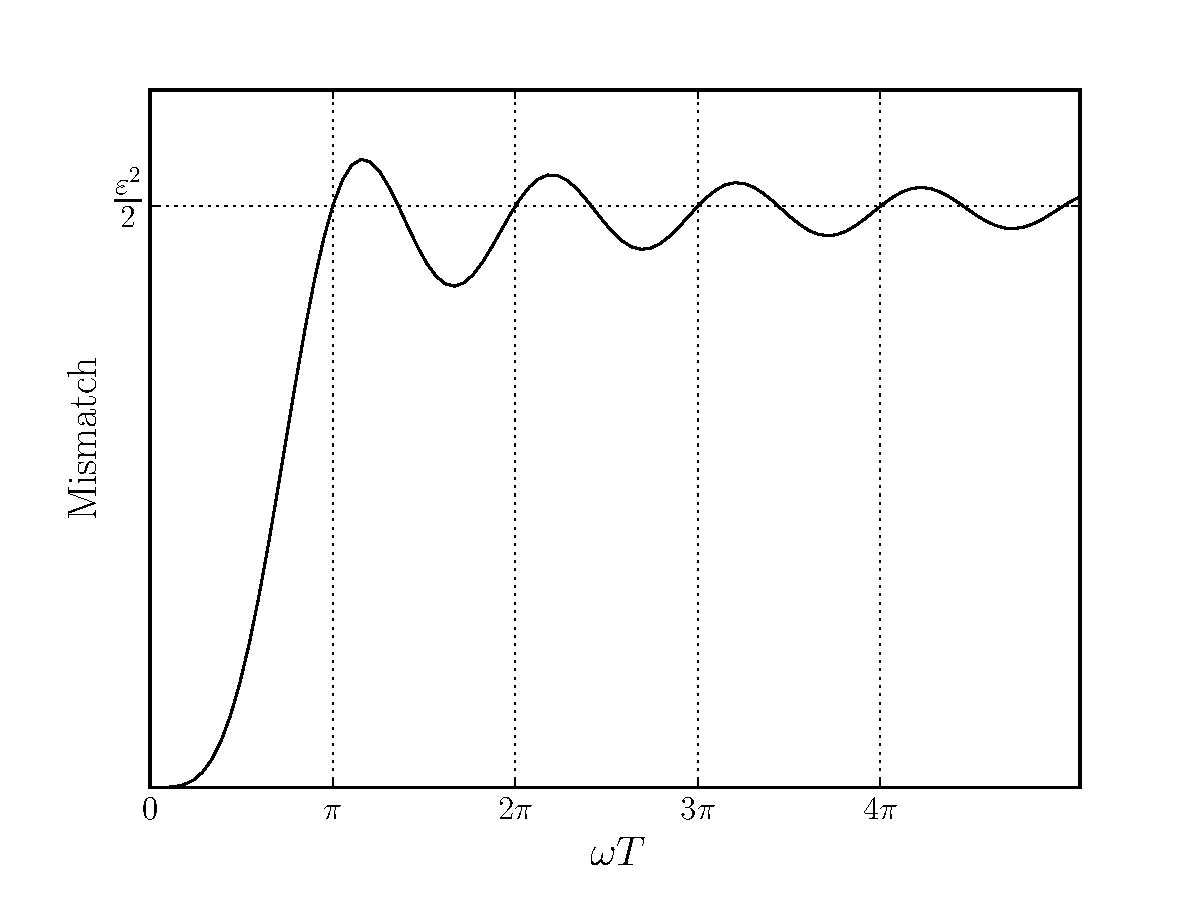
\includegraphics[width=.75\textwidth]{OscillatoryPhaseMismatch}
\caption{Plot demonstrating the behaviour of Eqn.~\eqref{eqn: Oscillating
mismatch}, the mismatch for an oscillating phase offset.}
\label{fig: OscillatoryPhaseMismatch}
\end{figure}

This simple model demonstrates that if the signal and template are on average
coherent, but the phase residual between them oscillates about the mean, then
over several cycles the mismatch will approach a constant value, which depends
on the maximum amplitude of the residuals.  For a quasi-periodic signal, we
expect the same overall picture will emerge with the size of the mismatch
dependent on the mean average size of oscillations in the residual.

\section{Generalising the metric-mismatch approximation to arbitrary signals}
\label{sec: generalising the metric-mismatch}

In the previous section, we discussed some special cases where the mismatch can be
calculated exactly for a signal which has a phase which can't be described by
a single Taylor expansion.
For more general signals, where the frequency and spin-down rate may
vary, the equations soon become unwieldy. In Section~\ref{sec: the
metric-mismatch approximation for fully-coherent searches} we introduced the
metric-mismatch, a tool to estimate the loss of SNR for Taylor expansion
signals and templates in fully-coherent searches. In this section, we will
extend the fully-coherent metric-mismatch to handle cases where the
signal is not a Taylor expansion, but can be approximated by a \emph{piecewise}
Taylor expansion; this will allow us to handle any arbitrary phase evolution of
the signal. By piecewise Taylor expansion we mean breaking any arbitrary signal into
$\Nsd$ \emph{subdomains} each of which we describe the signal by a single
Taylor expansion; the resulting collection of all individual Taylor expansions
is a piecewise Taylor expansion. We will distinguish between a \emph{subdomain}, which
describes a part of the piecewise function and a \emph{segment}, which is the division
of an observation period for a semi-coherent search as discussed in
Section~\ref{sec: semi-coherent mismatch}. 

This \emph{generalised metric-mismatch} will be used in Section~\ref{sec: glitches
in cgw} to calculate the mismatch due to glitches and in Section~\ref{sec: timing
noise in cgw analytic} to calculate the mismatch due to a random walk model of
timing noise.


%In this work we will be modelling glitches which can be described by a
%piecewise Taylor expansion with two subdomains. However, in this section we
%will develop a general formalism for a signal described by an arbitrary number
%$\Nsd$ subdomains.

\subsection{Piecewise Taylor expansion}
Before we get into the details of formulating a general metric-mismatch, it is
worth stating some details about piecewise Taylor expansions.
Allowing the signal to be piecewise amounts to placing a second index on the
signal parameters, $\ls^{\alpha a}$, which labels the subdomain of the piecewise function.
Note that we discriminate between
Greek indices, labelling the parameter components, and Roman indices which
label the subdomain.
For the $a^{th}$ subdomain of the piecewise function, we define $\tref^{a}$
as the reference time of the Taylor expansion in that subdomain. These can
be defined arbitrarily, although it is usual to either define them
relative to each subdomain, or at a fixed value for all the subdomains.
The piecewise signal function in the $a^{th}$ subdomain is then
\begin{align}
\PhiS(t; \{\ls^{\alpha a}\}) & = \phiS^a + 2\pi \left(\nuS^a (t - \tref^a)
+ \frac{\nudotS^a}{2}(t - \tref^a)^{2} \right),
\label{eqn: piecewise Taylor lambda signal}
\end{align}
when $t_{a} < t \le t_{a+1}$ and otherwise undefined: in future this condition will
be assumed.  By $\{\ls^{\alpha a}\}$ we indicate the set of all signal
parameters and by implication their reference times.

Since we will be calculating the phase difference between the signal and template
it is convenient to similarly make the template a piecewise function with
parameters $\lt^{\alpha a}$ such that
\begin{align}
\PhiT(t; \{\lt^{\alpha a}\}) = \phi^a + 2\pi \left(\nuT^a (t - \tref^a)
+ \frac{\nudotT^a}{2}(t - \tref^a)^{2} \right).
\label{eqn: piecewise Taylor lambda template}
\end{align}
Then we may write the parameter space difference as
$\dl^{\alpha a} = \ls^{\alpha a} - \lt^{\alpha a}$, where both the signal and
template must refer to the same reference time.

Since we have set up the template phase in Eqn.~\eqref{eqn: piecewise Taylor
lambda template} as a piecewise Taylor expansion, the template can
be any arbitrary function described by a piecewise Taylor expansion. However,
all current and planned searches use a single global Taylor expansion template.
To model this, we must introduce \emph{consistency relations}
which ensure that the local subdomains all lie along a single global template
with parameters $[\phiT, \nuT, \nudotT]$ defined at $\tref$. These consistency
relations may be written as
\begin{align}
\begin{split}
\phiT^a & = \phiT + \nuT(\tref^a - \tref) + \frac{\nudotT^{2}}{2}(\tref^a - \tref)^{2}, \\
\nuT^a & = \nuT + \nudotT(\tref^a - \tref), \\
\nudotT^a & = \nudotT.
\end{split}
\end{align}
Note the subtle distinction between $\tref$, the global reference time and
$\tref^{a}$ the reference time for the $a^{th}$ subdomain.

Finally, we can generalise Eqn.~\eqref{eqn: Delta Phi} for the phase difference
to the piecewise Taylor expansion description of the signal and template:
\begin{align}
\Delta\Phi^{a}(t)& =  \PhiS(t; \ls^{\alpha a}) - \PhiT(t; \lt^{\alpha a})\\
& = \Deltaphi^{a} + 2\pi\left(\Deltanu^{a}(t-\tref^{a})
+ \frac{\Deltanudot^{a}}{2}(t - \tref^{a})^{2}\right).
\end{align}

\subsection{The generalised metric-mismatch approximation for fully-coherent
            searches}

We will now generalise the metric-mismatch approximation first introduced by
\citet{Brady1998} to the case where the signal and template are piecewise
Taylor expansions. This calculation follows that given in Section~\ref{sec: the
metric-mismatch approximation for fully-coherent searches} with the addition
of an index labelling the subdomains.

Using a piecewise Taylor expansion
to describe the signal and template, the discrete nature of the phase offset
$\Delta\Phi^{a}$ allows us to partition the matched filtering amplitude due to
the additivity of integration on intervals. The matched filtering amplitude,
given the set of template parameters and parameter offsets $\{\lt^{\alpha a},
\dl^{\alpha a}\}$, is then
\begin{align}
X(\{\lt^{\alpha a}, \dl^{\alpha a}\}) & =
\frac{1}{\Tcoh}\int_{0}^{\Tcoh}e^{i \Delta \Phi(t)}dt  \\
& =  \frac{1}{\Tcoh}\sum_{c}^{\Nsd} \int_{t^{c}}e^{i \Delta \Phi^{c}}dt,
\end{align}
where the integration is taken over the bounds of the $c^{th}$ subdomain. The
mismatch, in this general formulation, is then defined by
\begin{equation}
\mutilde(\{\lt^{\alpha a}, \dl^{\alpha a}\}) =
 1 -  |X(\{\lt^{\alpha a}, \dl^{\alpha a}\})|^{2}
\end{equation}
The mismatch has a local minimum of zero when $\zero$. Expanding in powers of
$\dl^{\alpha a}$, the leading order term is
\begin{align}
\begin{split}
\mutilde(\{\lt^{\alpha a}, \dl^{\alpha a}\}) =
 & \frac{1}{2} \partial_{\alpha a} \partial_{\beta b}
                \mutilde(\{\lt^{\alpha a}, \dl^{\alpha a}\})
                \dl^{\alpha a}\dl^{\beta b},
\label{eqn: mismatch expansion}
\end{split}
\end{align}
where $\partial_{\alpha a} \equiv \partial_{\dl^{\alpha a}}$.  The metric in
this formalism is identified as
\begin{equation}
g_{\alpha\beta ab} =
\frac{1}{2} \partial_{\alpha a} \partial_{\beta b}
            \mutilde(\{\lt^{\alpha a}, \dl^{\alpha a}\})
            \zerolim.
\end{equation}
We can then define the fully-coherent \emph{generalised metric-mismatch} as
\begin{equation}
\mutilde(\{\lt^{\alpha a}, \dl^{\alpha a}\}) =
 g_{\alpha\beta ab} \dl^{\alpha a}\dl^{\beta b}.
\label{eqn: mismatch}
\end{equation}
On the right hand side we sum over the repeated indices. The mismatch is a
scalar value quantifying the loss of signal to noise due to the set of
parameter offsets~$\{\dl^{\alpha a}\}$.

Partially evaluating the metric we have
\begin{align}
\begin{split}
g_{\alpha\beta ab} = &  \frac{1}{\Tcoh}\sum_{c} \int_{t_{c}}
                        \partial_{\alpha a}\Delta \Phi^{c}
                        \partial_{\beta b}\Delta \Phi^{c}  dt\\
 & -
\frac{1}{\Tcoh^{2}}
\sum_{b} \int_{t_{c}}\partial_{\alpha a}\Delta \Phi^{c} dt
\sum_{b'} \int_{t_{c'}}\partial_{\beta c'}\Delta \Phi^{c'} dt.
\end{split}
\label{eqn: general metric}
\end{align}
Expanding the summation over the $a$ index, we note that,
\begin{equation}
 \partial_{\alpha a}\Delta \Phi^{c}  = \left[1, 2\pi (t - t_{r}^{a}),
                                           \pi (t - t_{r}^{a})^{2}
                                           \right]^{\alpha} \delta_{ac},
\label{eqn: NEterm}
\end{equation}
and so we can simplify Eqn.~\eqref{eqn: general metric} by dropping the terms
which vanish from the summation
\begin{align}
\begin{split}
g_{\alpha\beta ab} =& \frac{1}{\Tcoh}\delta_{ab} \int_{t_{a}}
                      \partial_{\alpha a}\Delta \Phi^{a}
                      \partial_{\beta a}\Delta \Phi^{a} dt \\
 & - \frac{1}{\Tcoh^{2}} \int_{t_{a}} \partial_{\alpha a}\Delta \Phi^{a} dt
  \int_{t_{b}} \partial_{\beta b}\Delta \Phi^{b} dt.
\end{split}
\label{eqn: metric}
\end{align}
This expression, given a choice of decomposition of the observation time $T$ into
$\Nsd$ (not necessarily equal) time subdomains labelled $t_{a}$, will result in a rank 4
tensor. Then, given a set of $\{\dl^{\alpha a}\}$ which together with the decomposition
of the time into subdomains defines the signal and template evolution, the
fully-coherent metric-mismatch can be calculated from Eqn.~\eqref{eqn: mismatch}.
%To help with the calculation we can also write out the term
%\begin{equation}
% \partial_{\alpha}\Delta \Phi^{i}  \partial_{\beta}\Delta \Phi^{i}  =
% \left[\begin{array}{ccc}
%1  & 2\pi (t - t_{r}^{i}) &  \cdots \\
%2\pi (t - t_{r}^{i}) & (2\pi)^{2} (t - t_{r}^{i})^{2} & \cdots \\
%2\pi (t - t_{r}^{i}) & (2\pi)^{2} (t - t_{r}^{i})^{2} & \cdots \\
%\vdots & \vdots & \ddots
%\end{array}
%\right]^{\alpha\beta}.
%\label{eqn: Eterm}
%\end{equation}
%In general calculating the metric requires the integration of each term in
%equations \eqref{eqn: Eterm} and \eqref{eqn: NEterm} with consideration given
%to the reference time

\subsection{Explicit calculation of the metric}
In this final subsection, we will derive two explicit calculation of the metric
given choices for the reference times. These will be used later on in this
thesis.
\subsubsection{Reference times in the middle of the subdomains}
If there are $\Nsd$
subdomains with the $a^{th}$ subdomain of duration $\dT_a$ then we can bound the
integration over each subdomain by $t_{a}, t_{a} + \dT_a$. We are free to choose
the reference time
in any way we like; for this example, we define the reference time in each subdomain
to be halfway through, that is $\tref^{a} = t_{a} + \dT_a/2$. Using the following identity
\begin{align}
\int_{t_{a}}^{t_{a}+\dT_a} \left(t - (t_{a} + \frac{\dT_a}{2})\right)^{n}
dt \equiv  \frac{\left(1
+(-1)^{n}\right)}{n+1}\left(\frac{\dT_a}{2}\right)^{n+1},
\end{align}
we have that
\begin{equation}
\int_{t_{a}}^{t_{a}+\dT_a} \partial_{\alpha}\Delta \Phi^{a}  \partial_{\beta}\Delta \Phi^{a} dt =  \left[\begin{array}{ccc}
\dT_a  & 0 &  \frac{\pi \dT_a^{3}}{12}\\
0 & \frac{\pi^{2}\dT_a^{3}}{3} &  0\\
\frac{\pi \dT_a^{3}}{12} & 0  &  \frac{\pi^{2}\dT_a^{5}}{80}\\
\end{array}
\right]^{\alpha\beta},
\end{equation}
and
\begin{equation}
\int_{t^{a}}^{t_{a}+\dT_a} \partial_{\alpha}\Delta \Phi^{a}  dt =
 \left[\dT, 0 , \frac{\pi \dT_a^{3}}{12} \right]^{\alpha}.
\end{equation}
which can be inserted into Eqn.~\eqref{eqn: metric} to calculate the metric.

The rank 4 metric $g_{\alpha\beta a b}$ is degenerate in the subdomain indices
$a$ and $b$ having only two distinct terms. We can distinguish these by either
$a=b$ or $a\ne b$. This allows to write the metric $g_{\alpha \beta a b}$
compactly as
\begin{align}
g_{\alpha\beta ij} = \left[\begin{array}{ccc}
\delta_{ab}\frac{\dT_a}{\Tcoh} -\left(\frac{\dT_a}{\Tcoh}\right)^{2}
& 0
& \frac{\delta_{ab}}{\Tcoh}\frac{\pi \dT_a^{3}}{12} - \frac{\pi \dT_a^{4}}{12\Tcoh^{2}}\\
0
& \delta_{ab}\frac{\pi^{2}\dT_a^{3}}{3\Tcoh}
&  0\\
\frac{\delta_{ab}}{\Tcoh}\frac{\pi \dT_a^{3}}{12} - \frac{\pi \dT_a^{4}}{12\Tcoh^{2}}
& 0
&  \frac{\delta_{ab}}{\Tcoh}\frac{\pi^{2}\dT_a^{5}}{80} -  \left(\frac{\pi \dT_a^{3}}{12 \Tcoh}\right)^{2} \\
\end{array}
\right]^{\alpha\beta}.
\label{eqn: metric tref half}
\end{align}

\subsubsection{Reference times at the start of each subdomain}
If instead we set the reference time to be at the start of each subdomain then,
following the method used to derive Eqn.~\eqref{eqn: metric tref half}, the
metric can be written compactly as
\begin{equation}
\medmuskip=0mu
\thinmuskip=1.5mu
\thickmuskip=0mu
g_{\alpha\beta ij}  =  \left[\begin{array}{ccc}
\delta_{ij}N^{-1}  -N^{-2}  &
\pi\dT \left( \delta_{ij}N^{-1} - N^{-2}\right)&
\frac{\dT^{2}\pi}{3} \left( \delta_{ij}N^{-1} - N^{-2}\right)\\
\pi\dT \left( \delta_{ij}N^{-1} - N^{-2}\right)&
\pi^{2}\dT^{2}\left(\delta_{ij}\frac{4N^{-1}}{3} - N^{-2}\right) &
\pi^{2}\dT^{3}\left(\delta_{ij}\frac{N^{-1}}{2} - \frac{N^{-2}}{3}\right) \\
\frac{\dT^{2}\pi}{3} \left( \delta_{ij}N^{-1} - N^{-2}\right) &
\pi^{2}\dT^{3}\left(\delta_{ij}\frac{N^{-1}}{2} - \frac{N^{-2}}{3}\right)  &
\pi^{2}\dT^{4}\left(\frac{N^{-1}}{5} - \frac{N^{-2}}{9}\right) \\
\end{array}
\right]^{\alpha, \beta}.
\label{eqn: metric equal subdomains tref 0}
\end{equation}



\biblio


\end{document}
